\documentclass[10pt,dvipdfmx]{beamer}
\usepackage{pgfpages}
\usepackage{graphicx}
\usepackage{listings,jlisting}
\usepackage{fancybox}
\usepackage{hyperref}
\usepackage{multimedia}

%%%%%%%%%%%%%%%%%%%%%%%%%%%
%%% themes
%%%%%%%%%%%%%%%%%%%%%%%%%%%
\usetheme{Rochester}
%% no navigation bar
% default boxes Bergen Boadilla Madrid Pittsburgh Rochester
%% tree-like navigation bar
% Antibes JuanLesPins Montpellier
%% toc sidebar
% Berkeley PaloAlto Goettingen Marburg Hannover Berlin Ilmenau Dresden Darmstadt Frankfurt Singapore Szeged
%% Section and Subsection Tables
% Copenhagen Luebeck Malmoe Warsaw

%%%%%%%%%%%%%%%%%%%%%%%%%%%
%%% innerthemes
%%%%%%%%%%%%%%%%%%%%%%%%%%%
% \useinnertheme{circles}	% default circles rectangles rounded inmargin

%%%%%%%%%%%%%%%%%%%%%%%%%%%
%%% outerthemes
%%%%%%%%%%%%%%%%%%%%%%%%%%%
% outertheme
% \useoutertheme{default}	% default infolines miniframes smoothbars sidebar sprit shadow tree smoothtree


%%%%%%%%%%%%%%%%%%%%%%%%%%%
%%% colorthemes
%%%%%%%%%%%%%%%%%%%%%%%%%%%
\usecolortheme{seahorse}
%% special purpose
% default structure sidebartab 
%% complete 
% albatross beetle crane dove fly seagull 
%% inner
% lily orchid rose
%% outer
% whale seahorse dolphin

%%%%%%%%%%%%%%%%%%%%%%%%%%%
%%% fontthemes
%%%%%%%%%%%%%%%%%%%%%%%%%%%
\usefonttheme{serif}  
% default professionalfonts serif structurebold structureitalicserif structuresmallcapsserif

%%%%%%%%%%%%%%%%%%%%%%%%%%%
%%% generally useful beamer settings
%%%%%%%%%%%%%%%%%%%%%%%%%%%
% 
\AtBeginDvi{\special{pdf:tounicode EUC-UCS2}}
% do not show navigation
\setbeamertemplate{navigation symbols}{}
% show page numbers
\setbeamertemplate{footline}[frame number]


%%%%%%%%%%%%%%%%%%%%%%%%%%%
%%% define some colors for convenience
%%%%%%%%%%%%%%%%%%%%%%%%%%%

\newcommand{\mido}[1]{{\color{green}#1}}
\newcommand{\mura}[1]{{\color{purple}#1}}
\newcommand{\ore}[1]{{\color{orange}#1}}
\newcommand{\ao}[1]{{\color{blue}#1}}
\newcommand{\aka}[1]{{\color{red}#1}}

\setbeamercolor{syntax}{bg=cyan!20!white}
\setbeamercolor{example}{bg=yellow!20!white}
\setbeamercolor{output}{bg=white}

%%%%%%%%%%%%%%%%%%%%%%%%%%%
%%% how to typset code
%%%%%%%%%%%%%%%%%%%%%%%%%%%

\lstset{language = python,
numbers = left,
numberstyle = {\tiny \emph},
numbersep = 10pt,
breaklines = true,
breakindent = 40pt,
frame = tlRB,
frameround = ffft,
framesep = 3pt,
rulesep = 1pt,
rulecolor = {\color{blue}},
rulesepcolor = {\color{blue}},
flexiblecolumns = true,
keepspaces = true,
basicstyle = \ttfamily\small,
identifierstyle = ,
commentstyle = ,
stringstyle = ,
showstringspaces = false,
tabsize = 4,
escapechar=\@,
xrightmargin=3zw,
}

\title{剛体の物理の基礎}
\institute{東京大学}
\author{田浦健次朗 \\ 電子情報工学科}
\date{}

\AtBeginSubsection[] % Do nothing for \section*
{
\begin{frame}
\frametitle{Contents}
\tableofcontents[currentsection,currentsubsection]
\end{frame}
}

\begin{document}
\maketitle

%%%%%%%%%%%%%%%%%%%%%%%%%%%%%%%%%% 
% \begin{frame}
% \frametitle{Contents}
% \tableofcontents
% \end{frame}

%%%%%%%%%%%%%%%%% 
% \begin{frame}[fragile]
% \frametitle{以下のスライド}
% 以下のスライドで,
% \begin{beamercolorbox}{syntax}
% 青地で囲まれているのは, 文法規則の説明
% \end{beamercolorbox}

% \begin{beamercolorbox}{example}
% 緑地で囲まれているのは, プログラム例
% \end{beamercolorbox}

% \begin{beamercolorbox}{output}
% 黄地で囲まれているのは, プログラムを実行した際の出力
% \end{beamercolorbox}
% \end{frame}

%%%%%%%%%%%%%%%%% %%%%%%%%%%%%%%%%% 
\section{}

%%%%%%%%%%%%%%%%% %%%%%%%%%%%%%%%%% 
\begin{frame}
\frametitle{目標}
剛体の運動をシミュレーションできるようになるための基礎

\begin{itemize}
\item さしあたり問題19ができるようになる
\item ただし, 
より一般の場合にも通用するための理論を身につける
\end{itemize}

\end{frame}


%%%%%%%%%%%%%%%%% %%%%%%%%%%%%%%%%% 
\begin{frame}
\frametitle{剛体の運動のとらえ方}
剛体: 変形しない
\begin{columns}
\begin{column}{0.6\textwidth}
\begin{itemize}
\item $\Rightarrow$ 剛体内の各点の「速度」は,
\begin{enumerate}
\item \aka{「ある基準点」の速度}
\item \aka{その基準点を中心とした回転}
\end{enumerate}
だけで決まる

\item 注: 回転は「その基準点を中心」とするもの以外は考えられないことに注意
  \begin{itemize}
  \item[] \footnotesize{基準点と一緒に動く観察者を想像してみよ. その観察者から見て,
      基準点は静止しているわけだから, 
      残る動きは, その基準点が動かないような($=$その基準点を中心とした)
      回転だけである.}
  \end{itemize}
\end{itemize}
\end{column}

\begin{column}{0.4\textwidth}
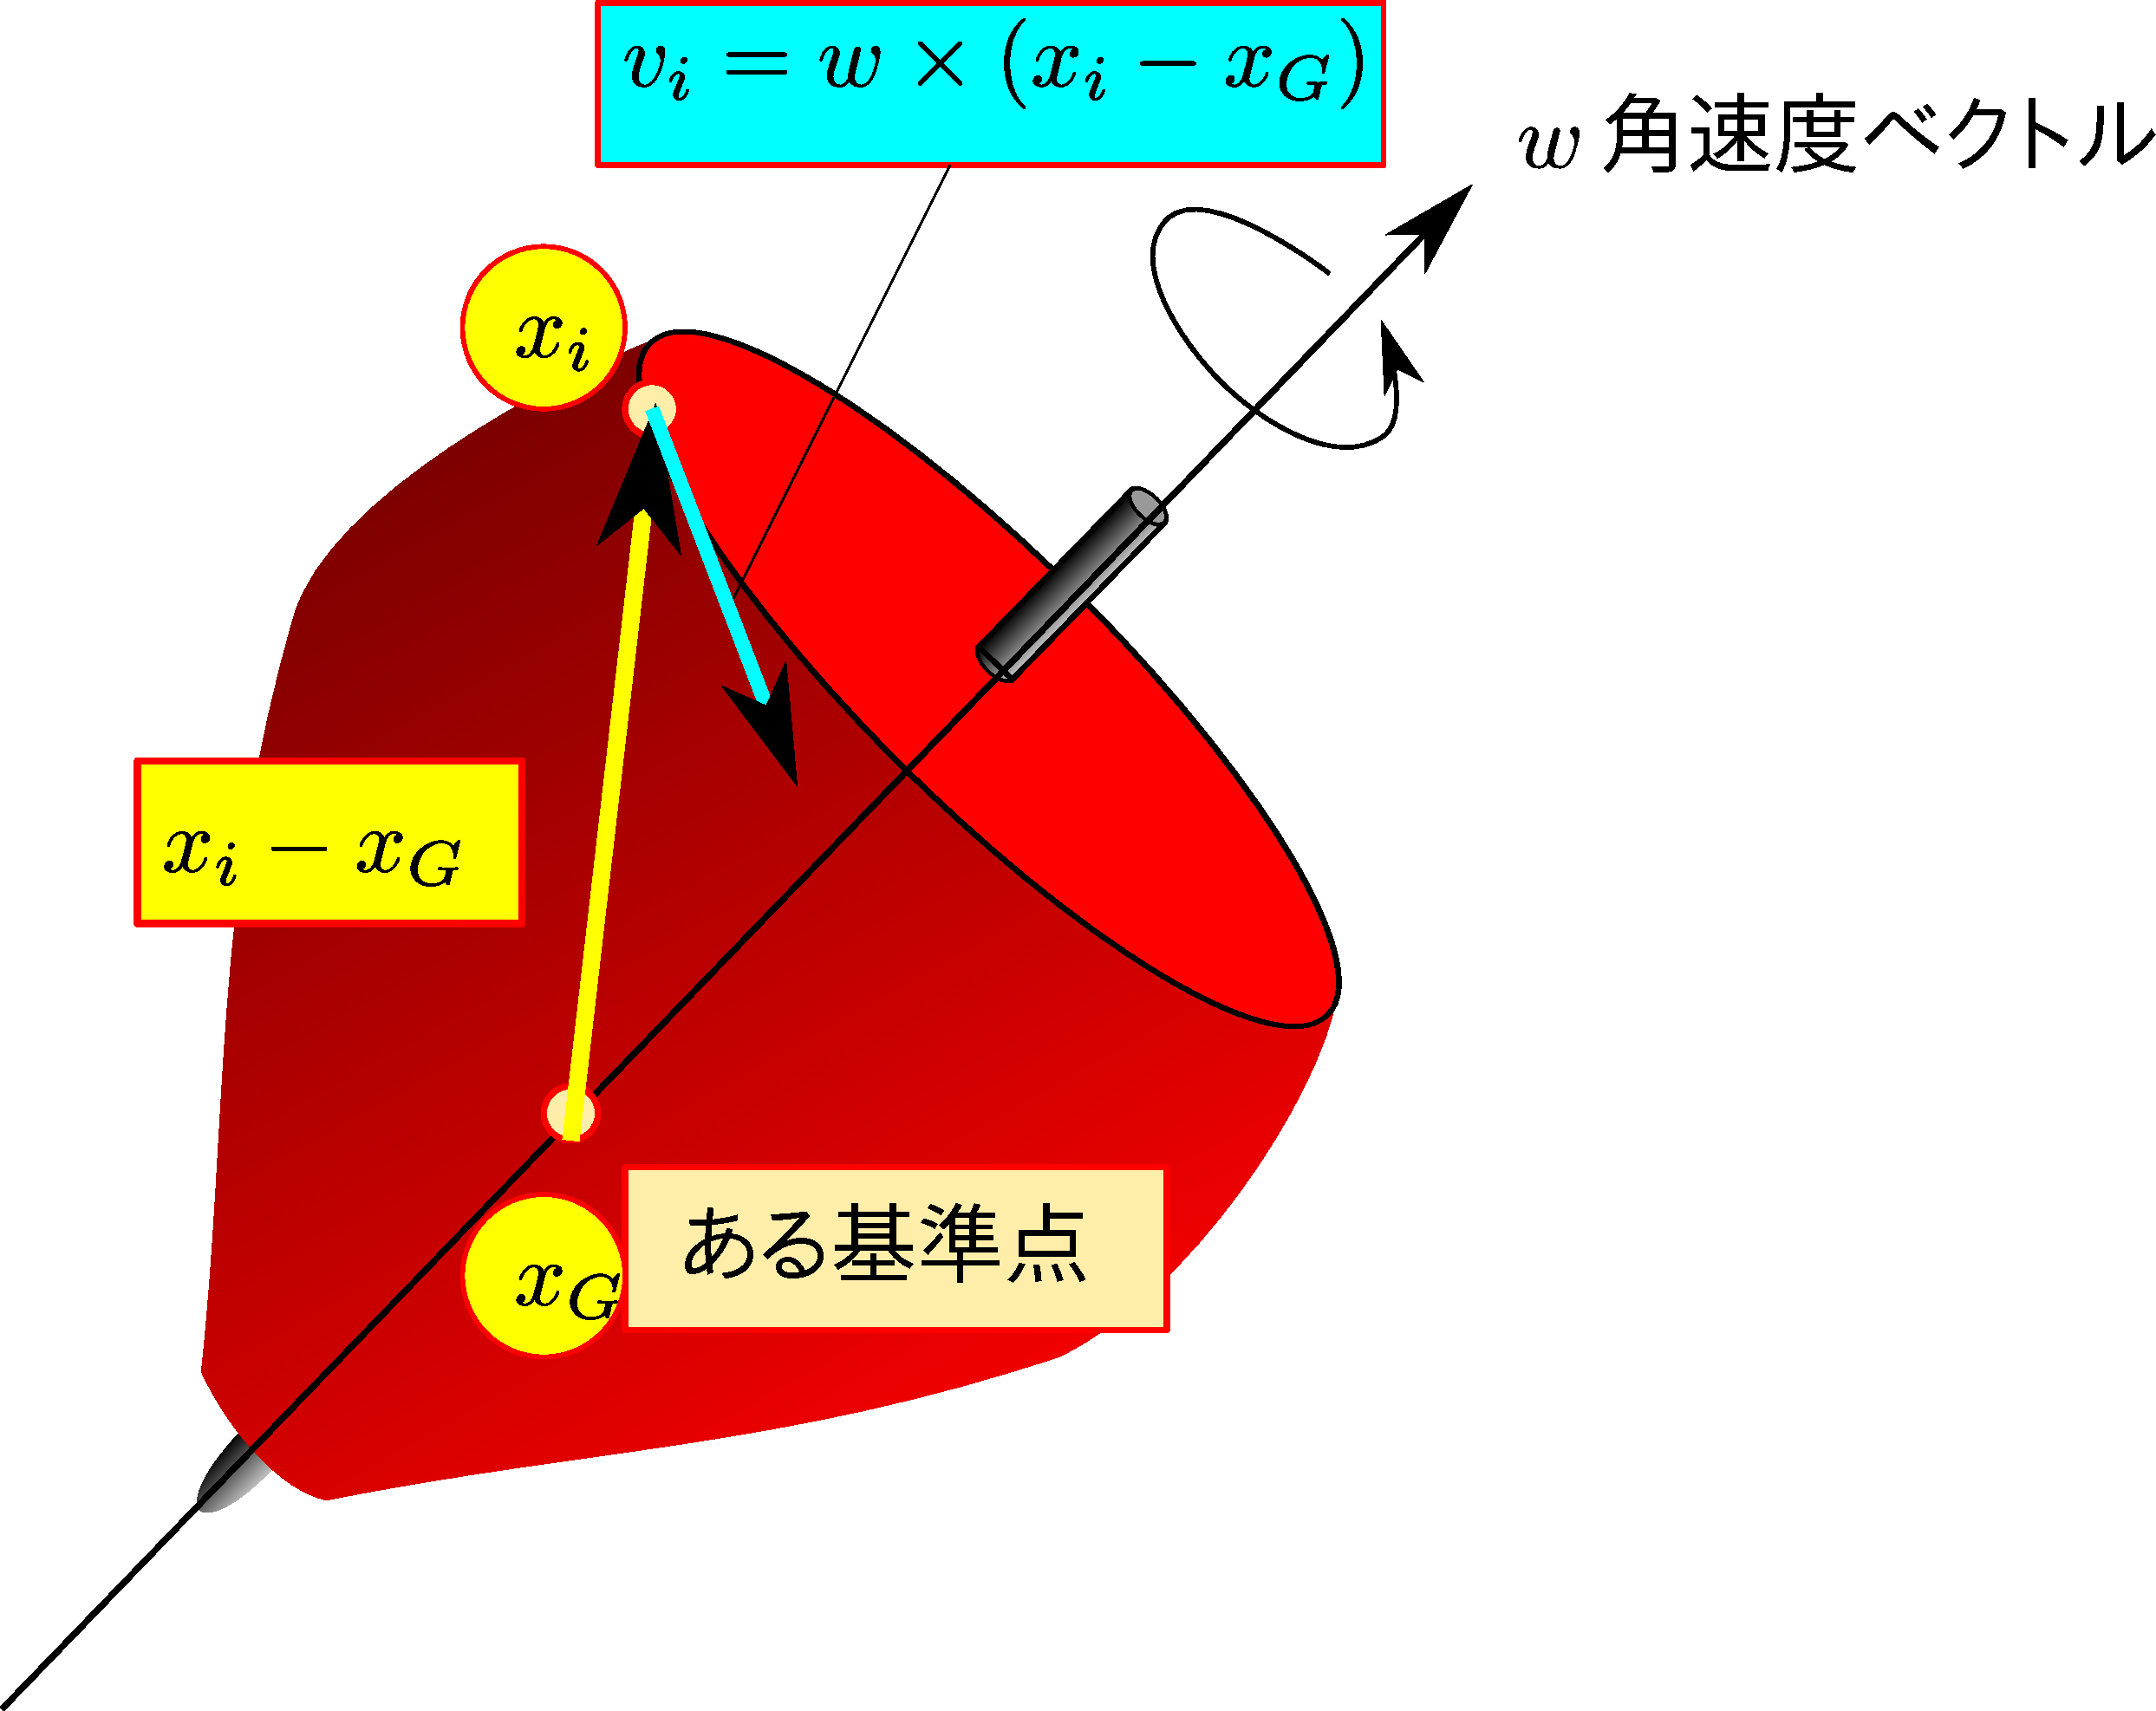
\includegraphics[width=\textwidth]{out/pdf/svg/v_w_r.pdf}
\end{column}

\end{columns}
\end{frame}


%%%%%%%%%%%%%%%%% %%%%%%%%%%%%%%%%% 
\begin{frame}
\frametitle{剛体の運動のとらえ方}
\begin{columns}
\begin{column}{0.6\textwidth}
\begin{itemize}
\item 剛体内の各点の「速度」は,
\begin{enumerate}
\item \aka{「ある基準点」の速度}
\item \aka{その基準点を中心とした回転}
\end{enumerate}
だけで決まる

\item より具体的には, 剛体内の点$i$の速度$v_i$は,
\aka{
  \begin{equation}
v_i = v_G + w \times (x_i - x_G) \label{eq:v_w_r}
  \end{equation}}
となる(右図を見て納得せよ)
\begin{itemize}
\item $x_i$ : 点$i$の位置
\item $v_G$, $x_G$ : 「ある基準点」の位置, 速度
\item $w$ : 角速度ベクトル\aka{(剛体全体で共通)}
\end{itemize}
\end{itemize}
\end{column}

\begin{column}{0.4\textwidth}
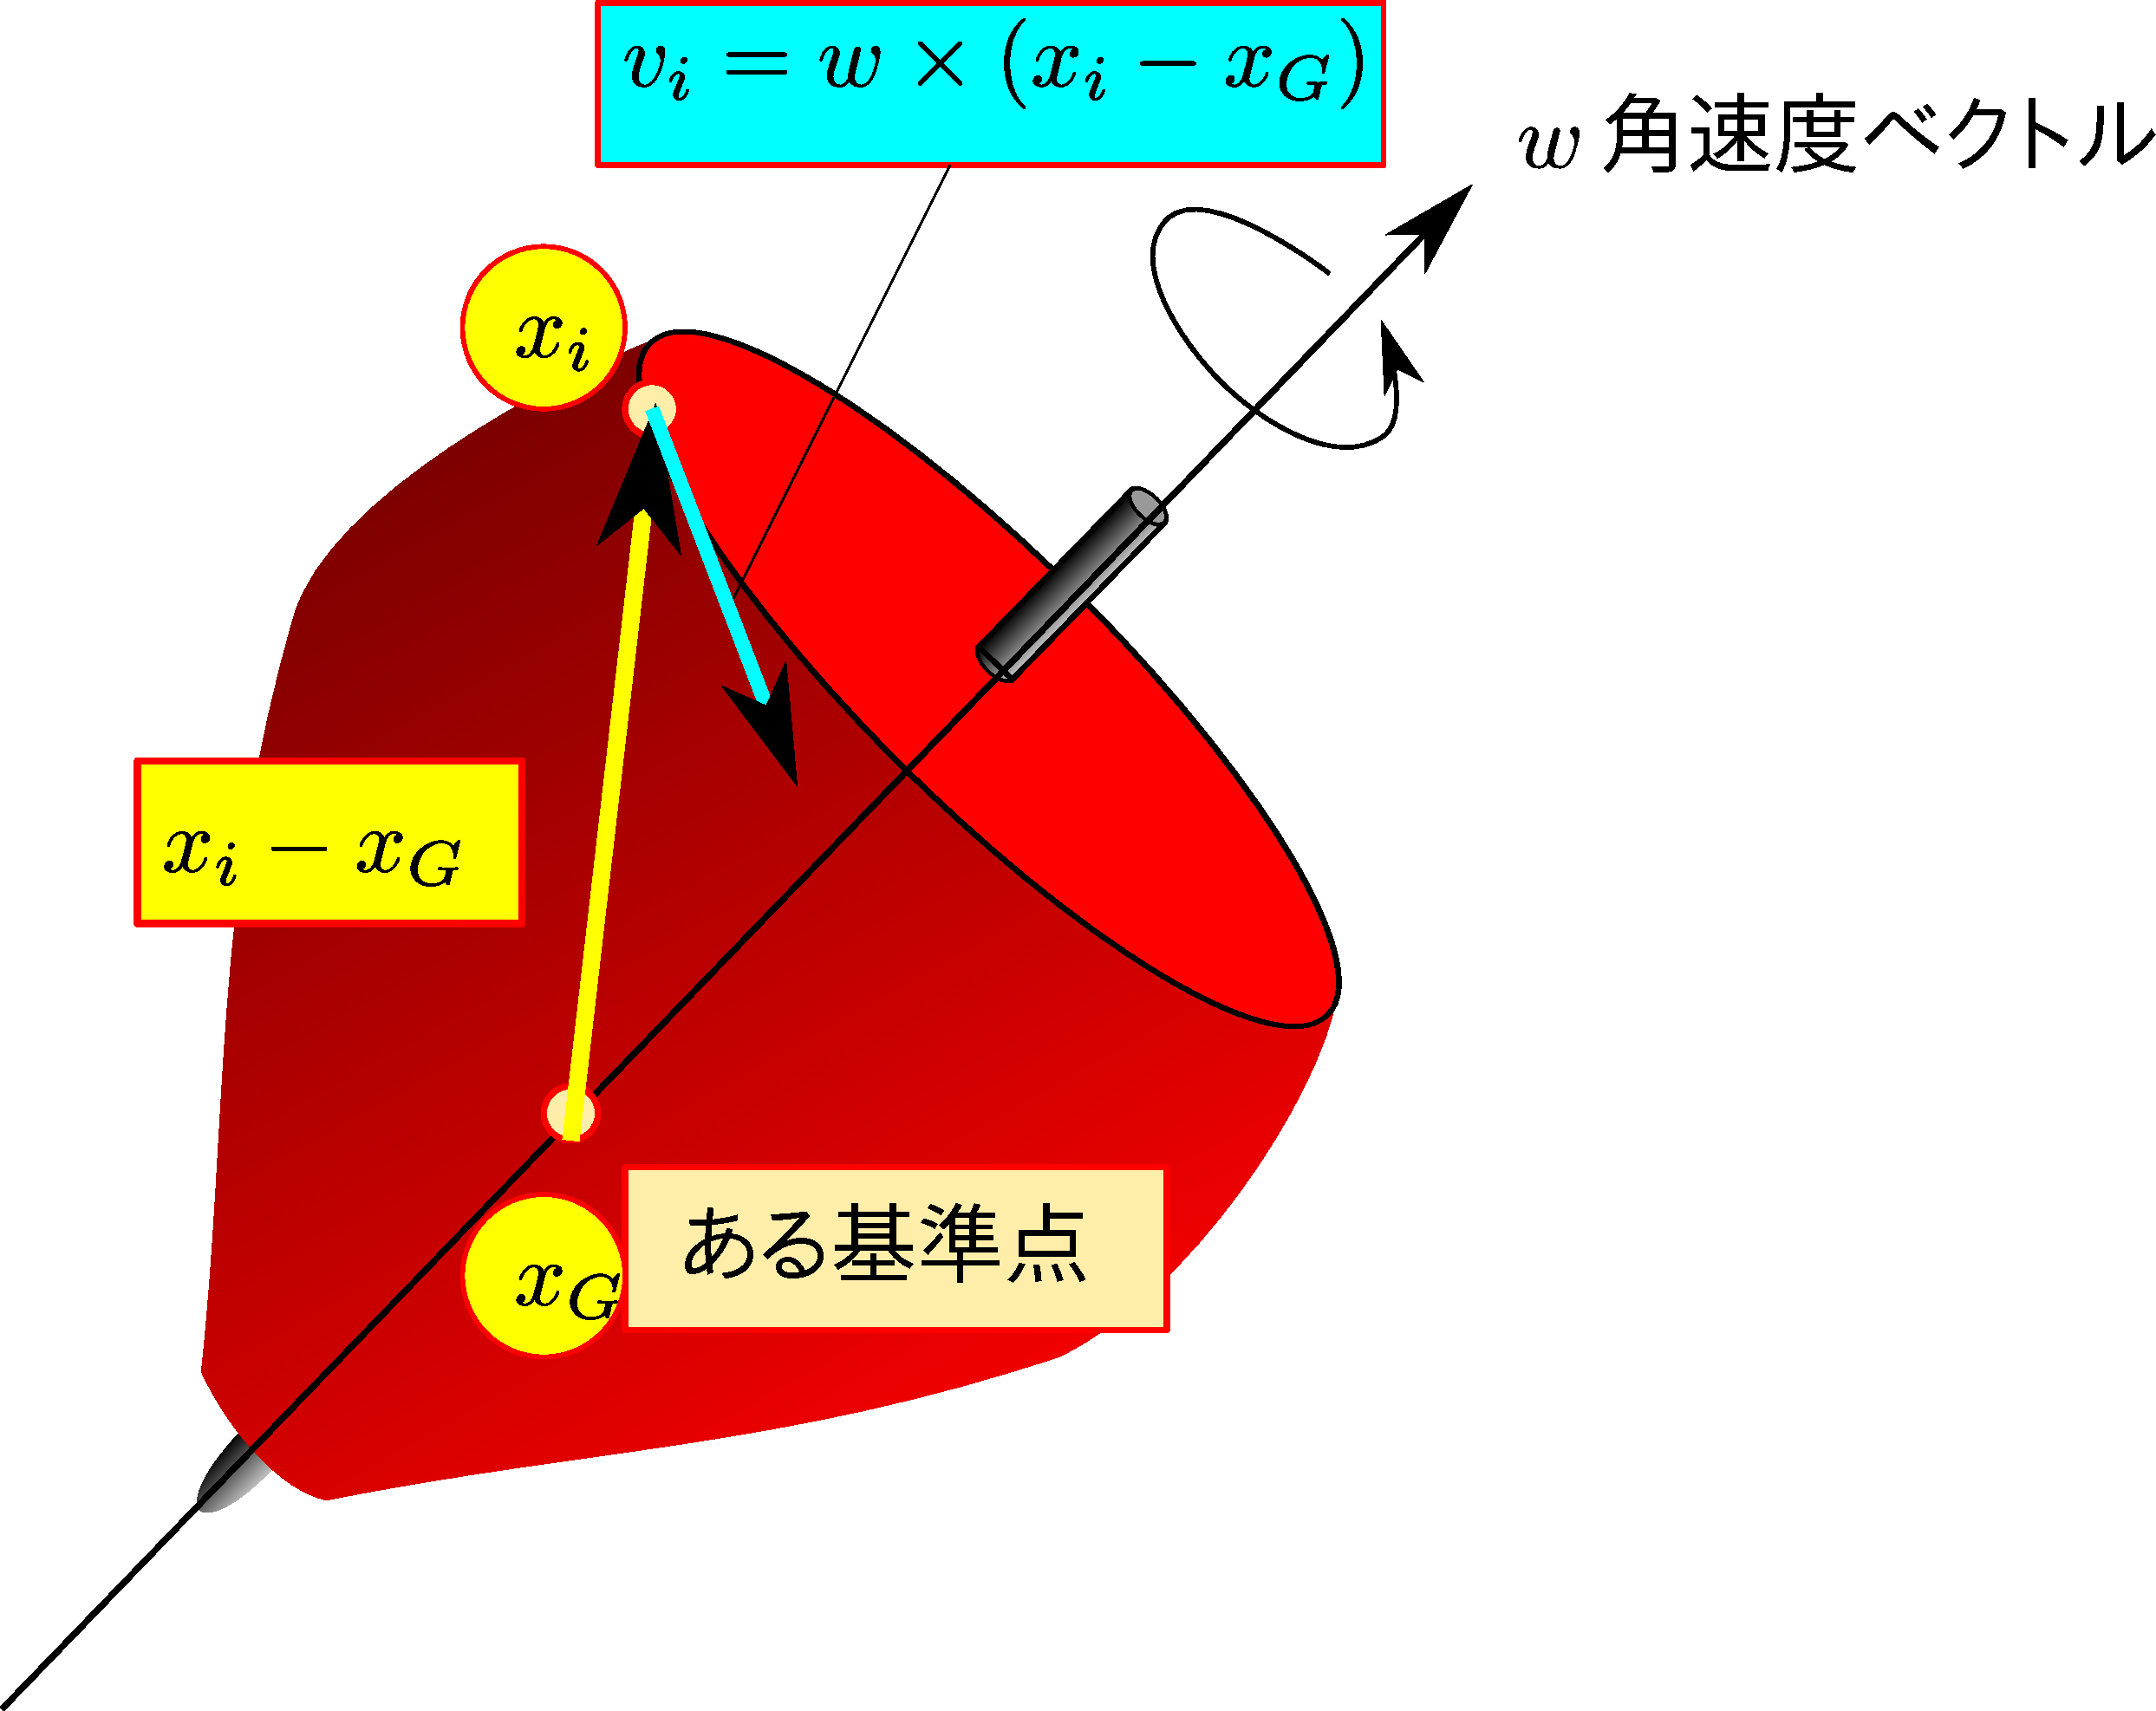
\includegraphics[width=\textwidth]{out/pdf/svg/v_w_r.pdf}
\end{column}
\end{columns}

\scriptsize{つまり, 「ある基準点」の位置, 速度がきまり,
あとは$w$という一つのベクトル(角速度ベクトル)さえ決まってしまえば,
剛体を構成する「全ての」点の速度が決まってしまう.
点の速度が決まれば点の位置も追跡できるわけだから,
結局, 「ある基準点」の位置, 速度, および, 
角速度ベクトル$w$さえ追跡できれば良いという事になる}


\end{frame}

%%%%%%%%%%%%%%%%% %%%%%%%%%%%%%%%%% 
\begin{frame}
\frametitle{注: 角速度はベクトル}
\begin{columns}
\begin{column}{0.6\textwidth}
\begin{itemize}
\item 3次元空間内の一般の運動では角速度はベクトル
  \begin{enumerate}
  \item ベクトルの方向は, 回転軸の方向
  \item ベクトルの大きさは回転の速さ
  \item ベクトルの向きは回転の向き
  \end{enumerate}
を, それぞれ示している(右ネジの向き)

\item 平面内の運動の場合, スカラーと思っても良い
  \begin{itemize}
  \item $xy$平面内の運動なら, 角速度は$z$軸方向のベクトル
  \item $\Rightarrow$ $z$成分だけを考えれば良い
  \end{itemize}
\end{itemize}
\end{column}

\begin{column}{0.4\textwidth}
  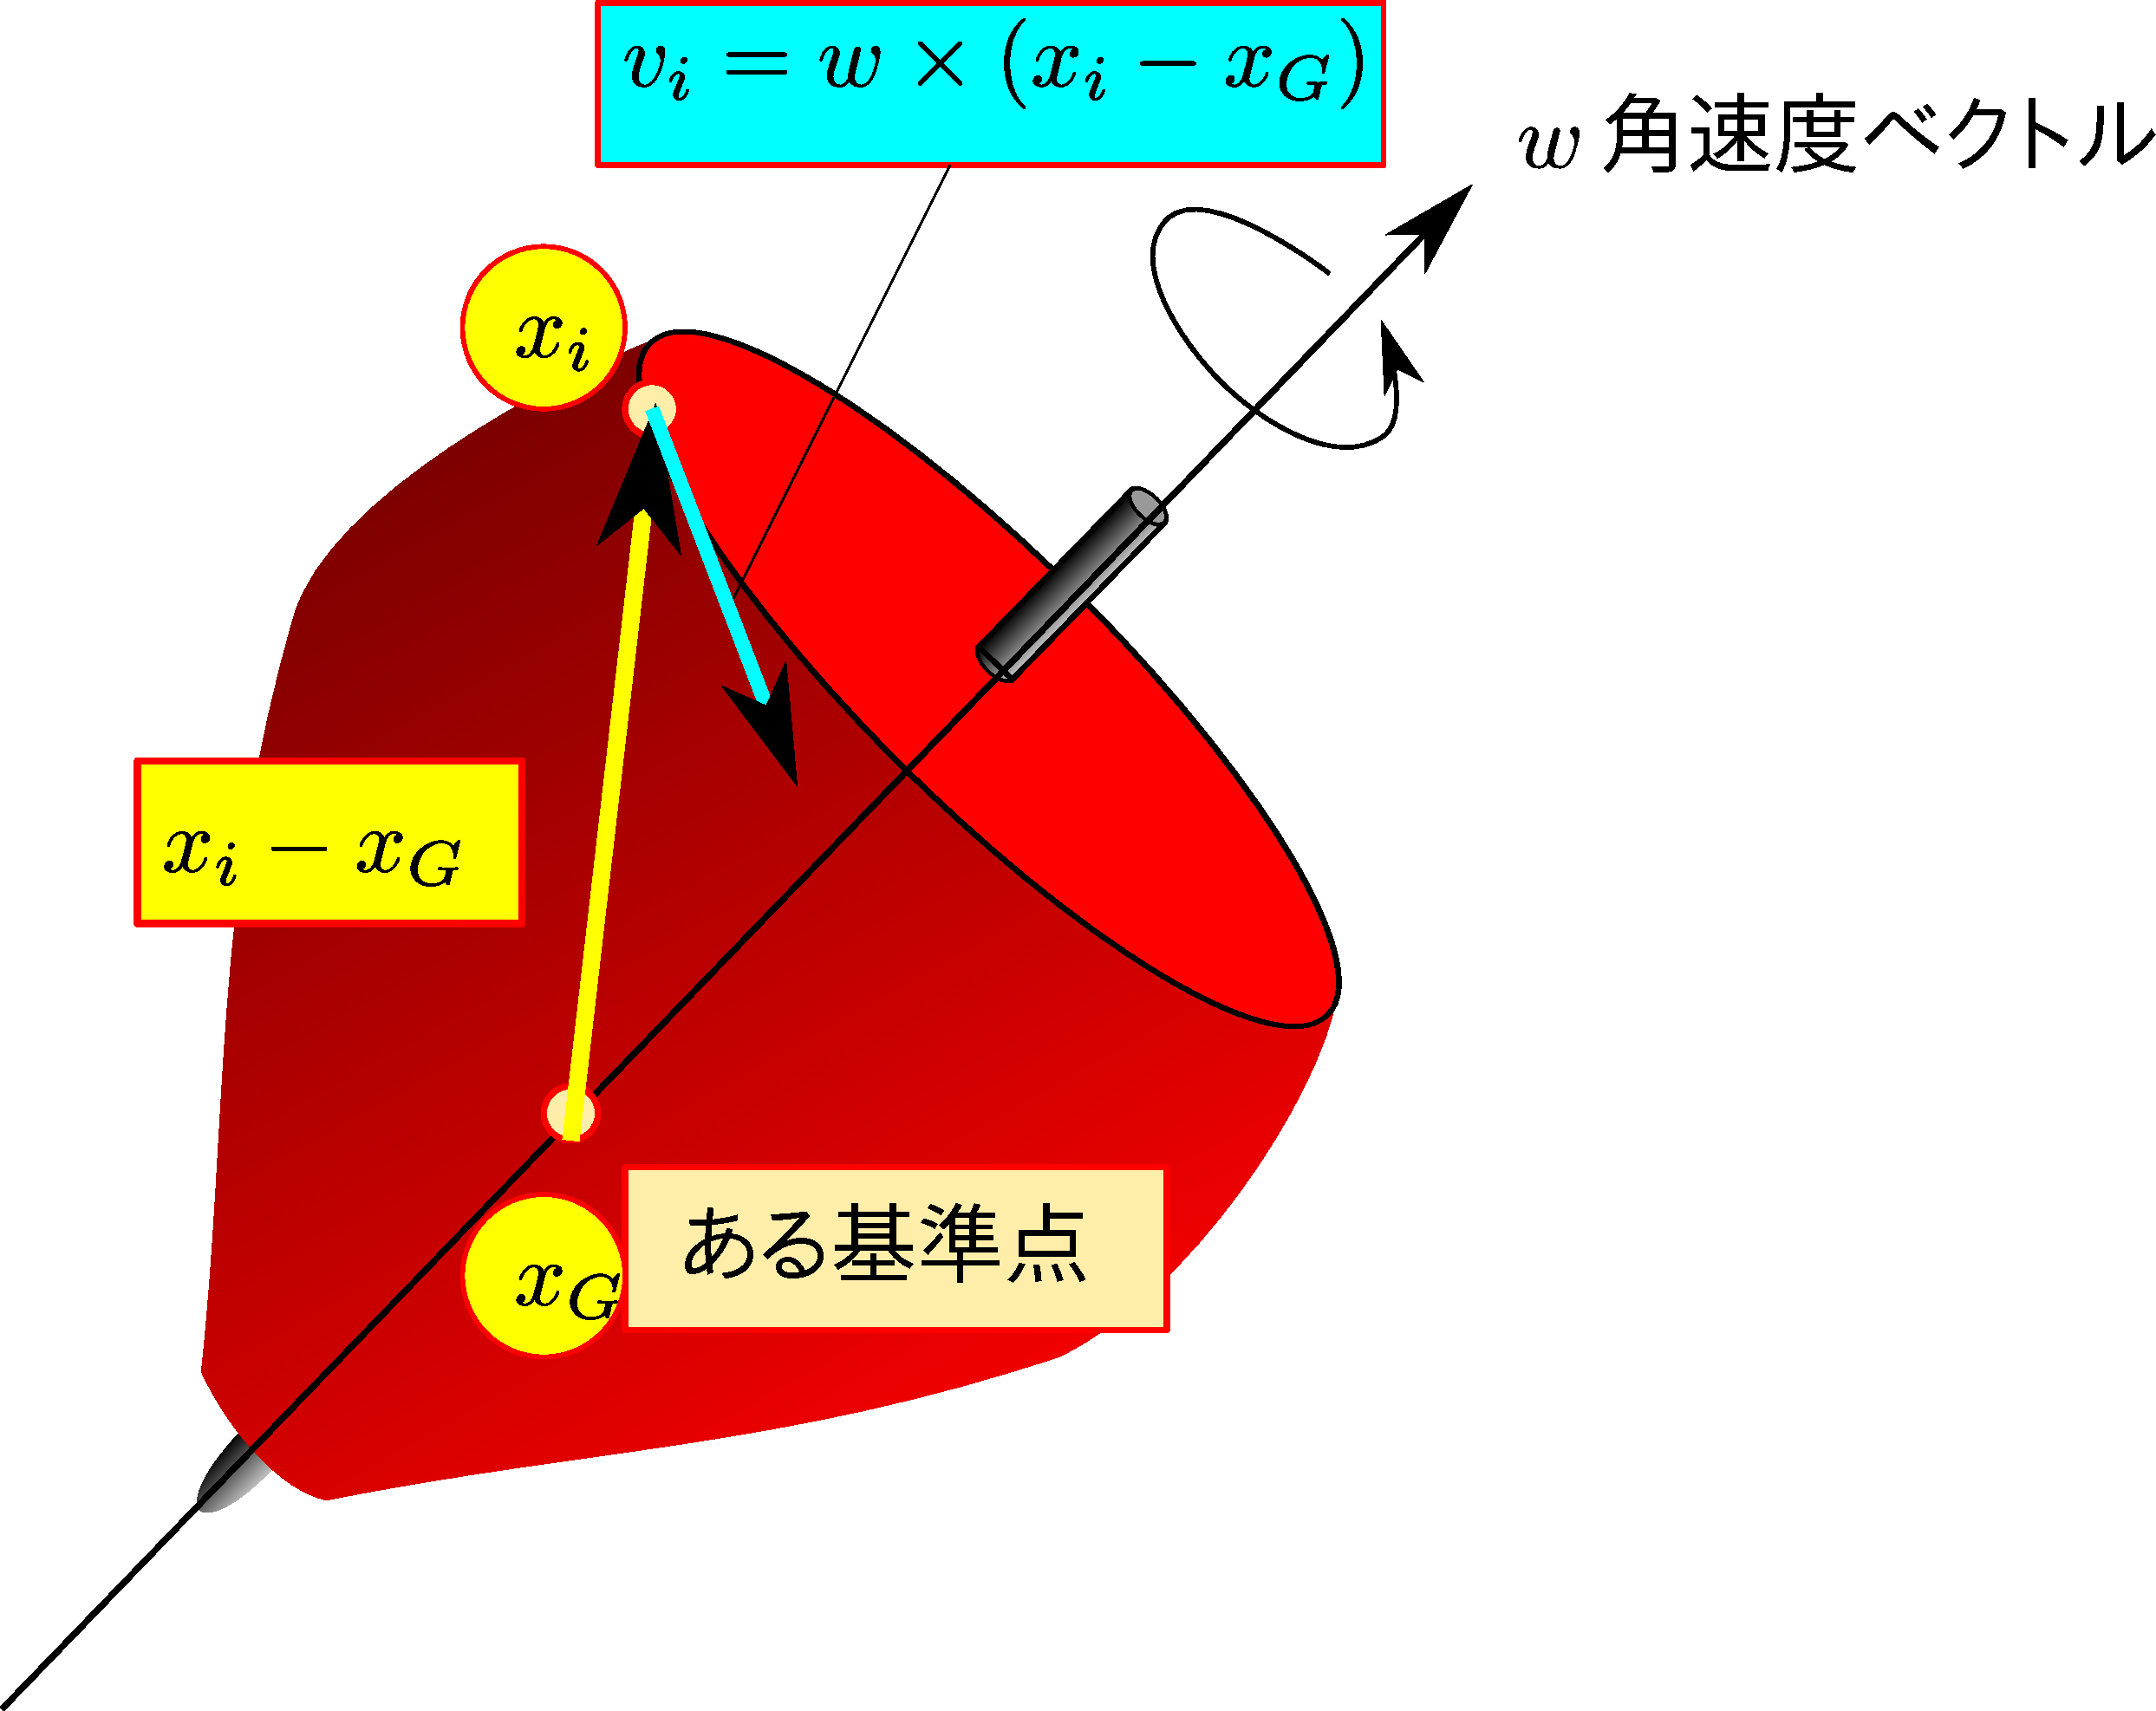
\includegraphics[width=\textwidth]{out/pdf/svg/v_w_r.pdf}
\end{column}
  
\end{columns}
\end{frame}

%%%%%%%%%%%%%%%%% %%%%%%%%%%%%%%%%% 
\begin{frame}
\frametitle{剛体の運動$=$「基準点」の運動$+$その周りの回転}

\begin{columns}
\begin{column}{0.6\textwidth}
\begin{itemize}
\item \ldots ということでこれから,
\begin{itemize}
\item \aka{「ある基準点」の運動}と,
\item \aka{その基準点の周りの角速度}
\end{itemize}
の追跡方法を見ていく

\item その前に, 「ある基準点」をどこにするか?
\begin{itemize}
\item ここまでの話では「何でも良い」
\item しかし, 「質量の中心」を使うと色々と話が簡単になる(ことがすぐにわかる)
\end{itemize}
\end{itemize}
\end{column}

\begin{column}{0.4\textwidth}
  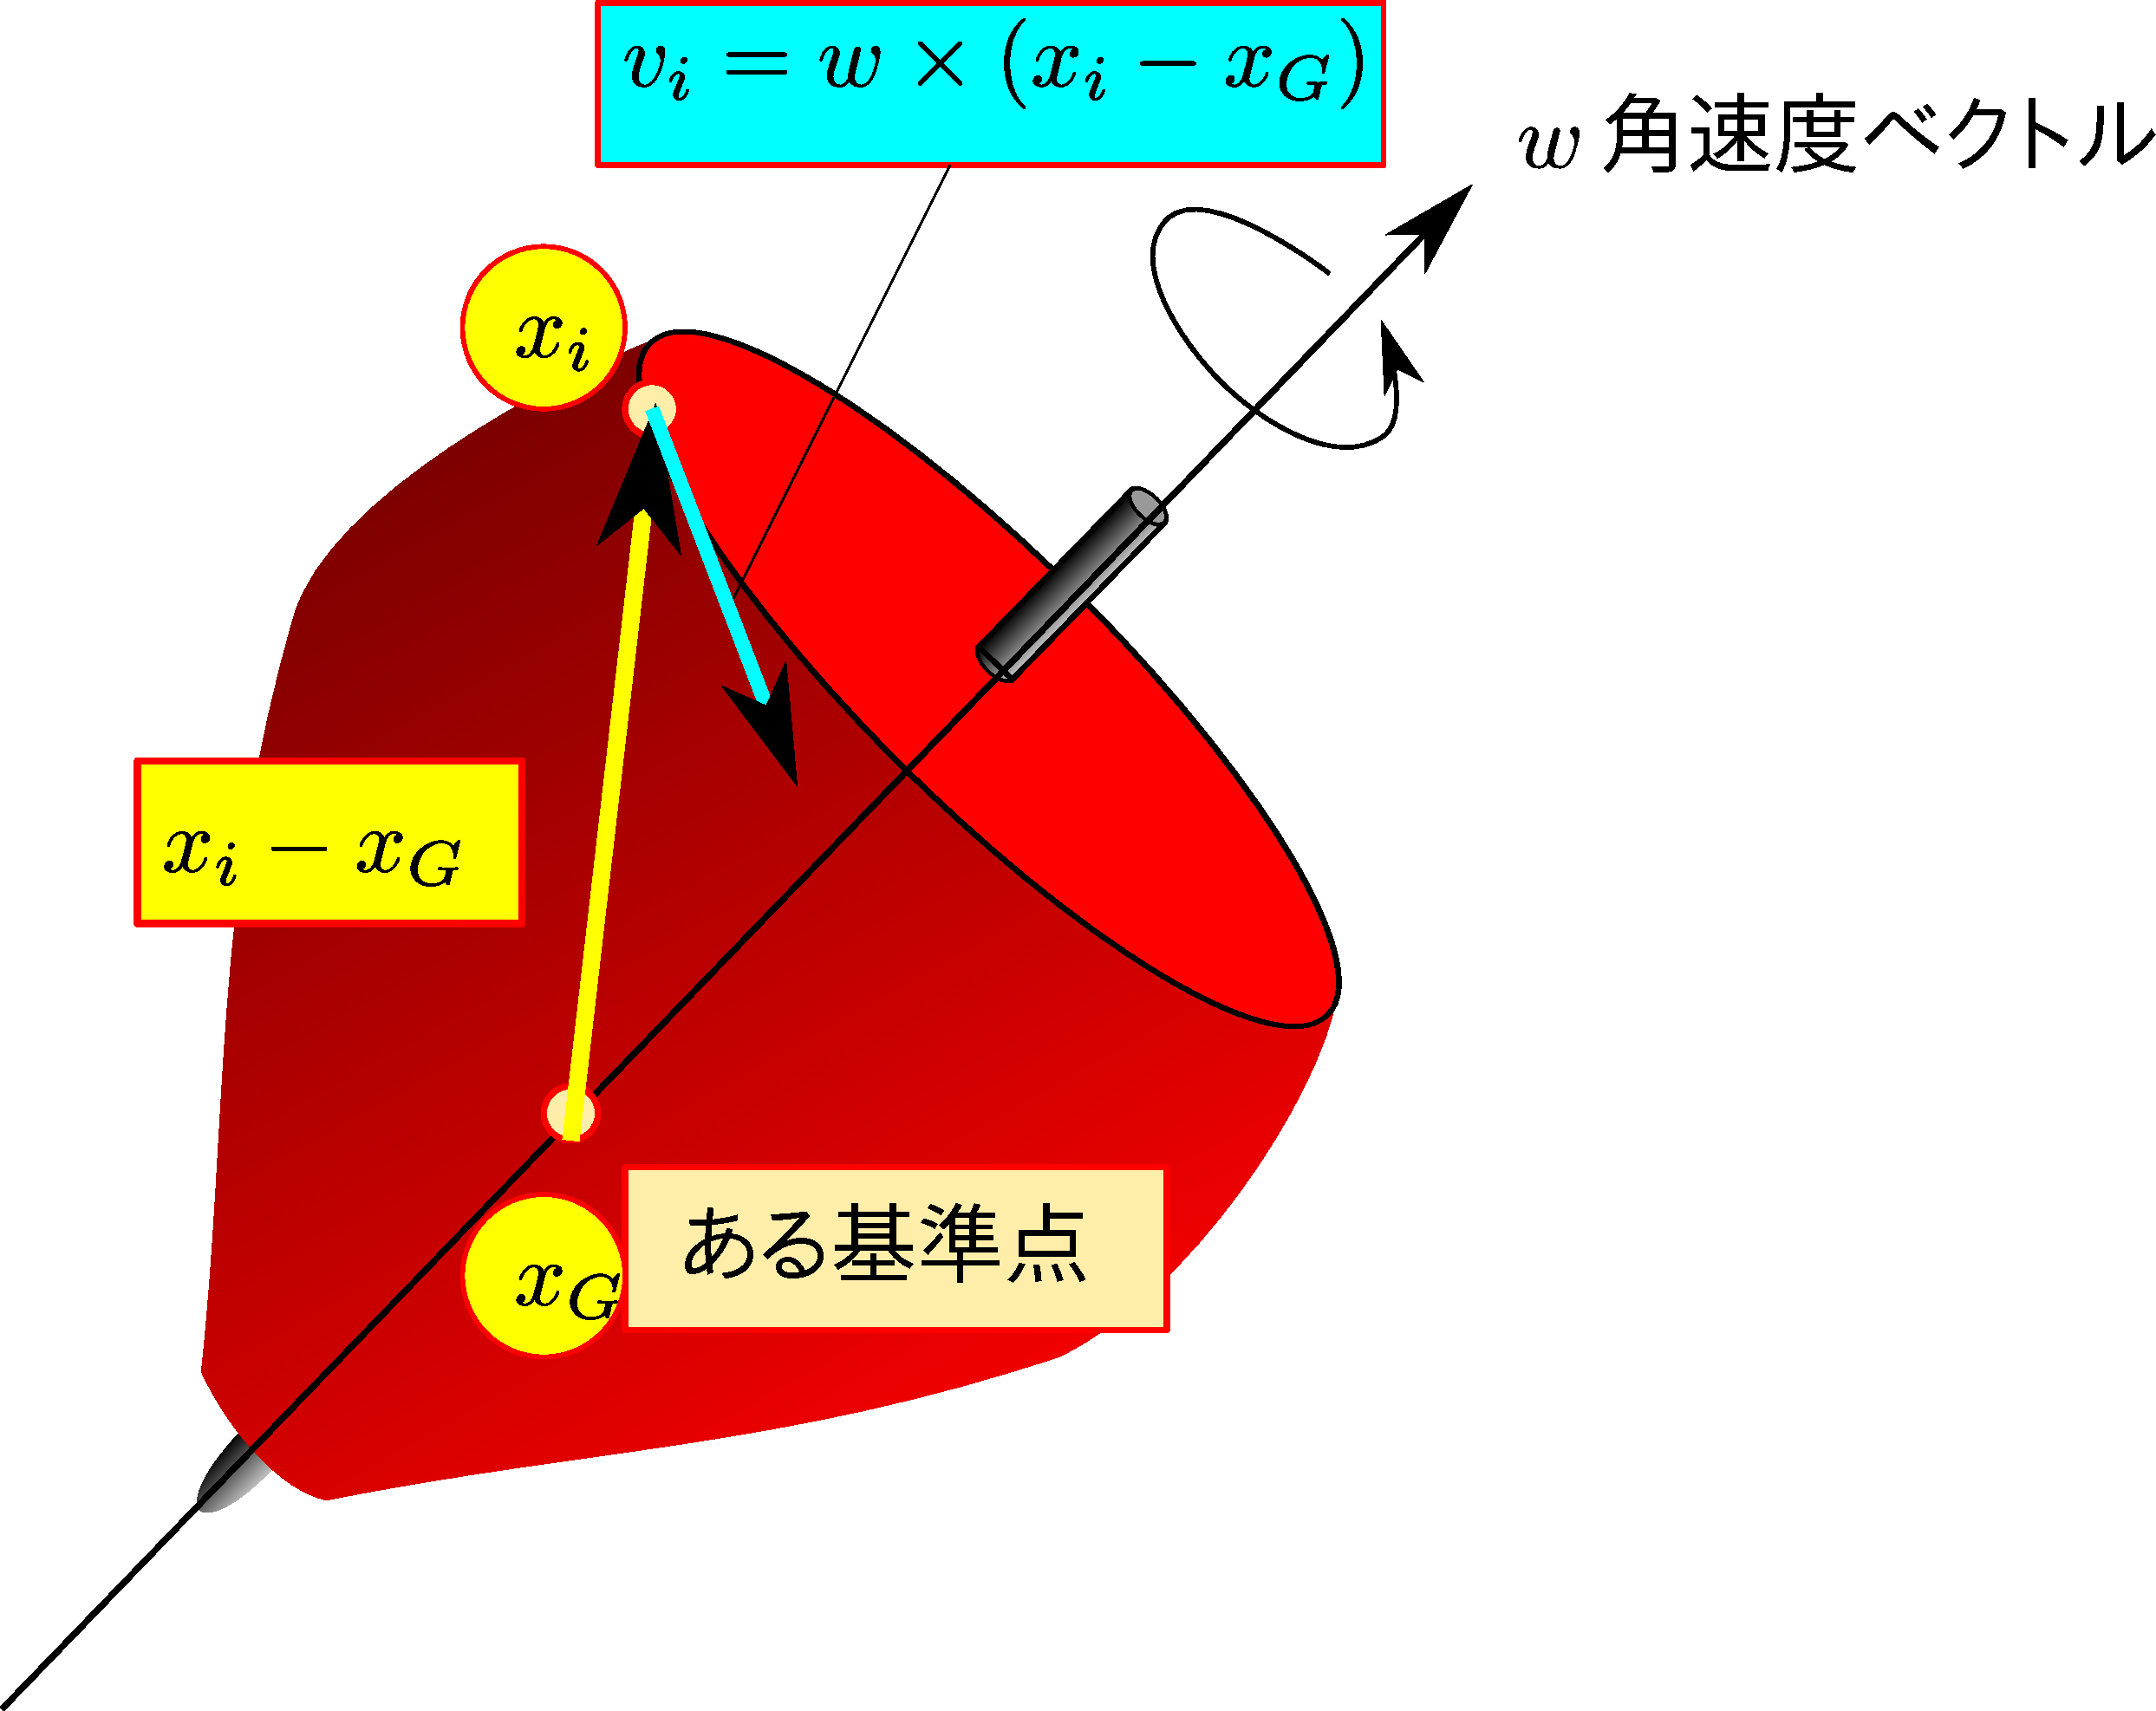
\includegraphics[width=\textwidth]{out/pdf/svg/v_w_r.pdf}
\end{column}
\end{columns}

\end{frame}

%%%%%%%%%%%%%%%%% %%%%%%%%%%%%%%%%% 
\begin{frame}[fragile]
\frametitle{「ある基準点」の運動}
先に前者を片付けておこう

\begin{itemize}
\item 点$i$の運動方程式:
\[ m_i \ddot{x_i} = f_i \]
\item 全部の点にわたり和をとる:
\[ \sum_i m_i \ddot{x_i} = \sum_i f^{\mbox{ext}}_i \]
\begin{itemize}
\item \scriptsize{$f^{\mbox{ext}}_i$は外力(内力は打ち消し合って0になるから)}
\item 以降, ${}^{\mbox{ext}}$は省略
\end{itemize}

\item 
\[ \therefore \aka{M \ddot{x}_G = \sum_i f_i} \]
\begin{itemize}
\item[] ここで,
\begin{eqnarray*}
M   & = & \sum_i m_i \;\mbox{(総質量)}, \\
x_G & = & \frac{\sum_i m_i x_i}{\sum_i m_i} \;\mbox{\aka{(質量中心)}の位置.} 
\end{eqnarray*}
\end{itemize}
\end{itemize}
\end{frame}

%%%%%%%%%%%%%%%%% %%%%%%%%%%%%%%%%% 
\begin{frame}[fragile]
\frametitle{質量中心の運動}

\begin{eqnarray*}
M \ddot{x}_G & = & \sum_i f_i
\end{eqnarray*}

\begin{itemize}
\item つまり質量の中心($x_G$)は, あたかも, そこにある質点が全ての外力を受けた場合と同じ動きをする
  \begin{itemize}
  \item 質量中心の動きに関しては, 質点の物理以上のものはいらない
  \item であれば「ある基準点」として質量中心を取りましょう!
  \end{itemize}
\item こうして, 後は質量中心の周りの回転(つまり角速度)を追跡できれば良いということになった
\end{itemize}

\end{frame}

%%%%%%%%%%%%%%%%% %%%%%%%%%%%%%%%%% 
\begin{frame}[fragile]
\frametitle{角速度の追跡}

\ao{角速度}の変化を求めるには, 
\aka{「角運動量」}なる量を媒介するとうまくいく.

考え方:
\begin{enumerate}
\item 剛体が「力」を受けると「角運動量」なるものが変化する
\item 「角運動量」と「角速度」の間には簡単な関係が存在する
\item 以上から, 力を受けた時角速度がどう変化するかがわかる
\end{enumerate}

次ページの図を参照.

\end{frame}

%%%%%%%%%%%%%%%%% %%%%%%%%%%%%%%%%% 
\begin{frame}
\frametitle{角速度の時間変化を追うためのロードマップ}

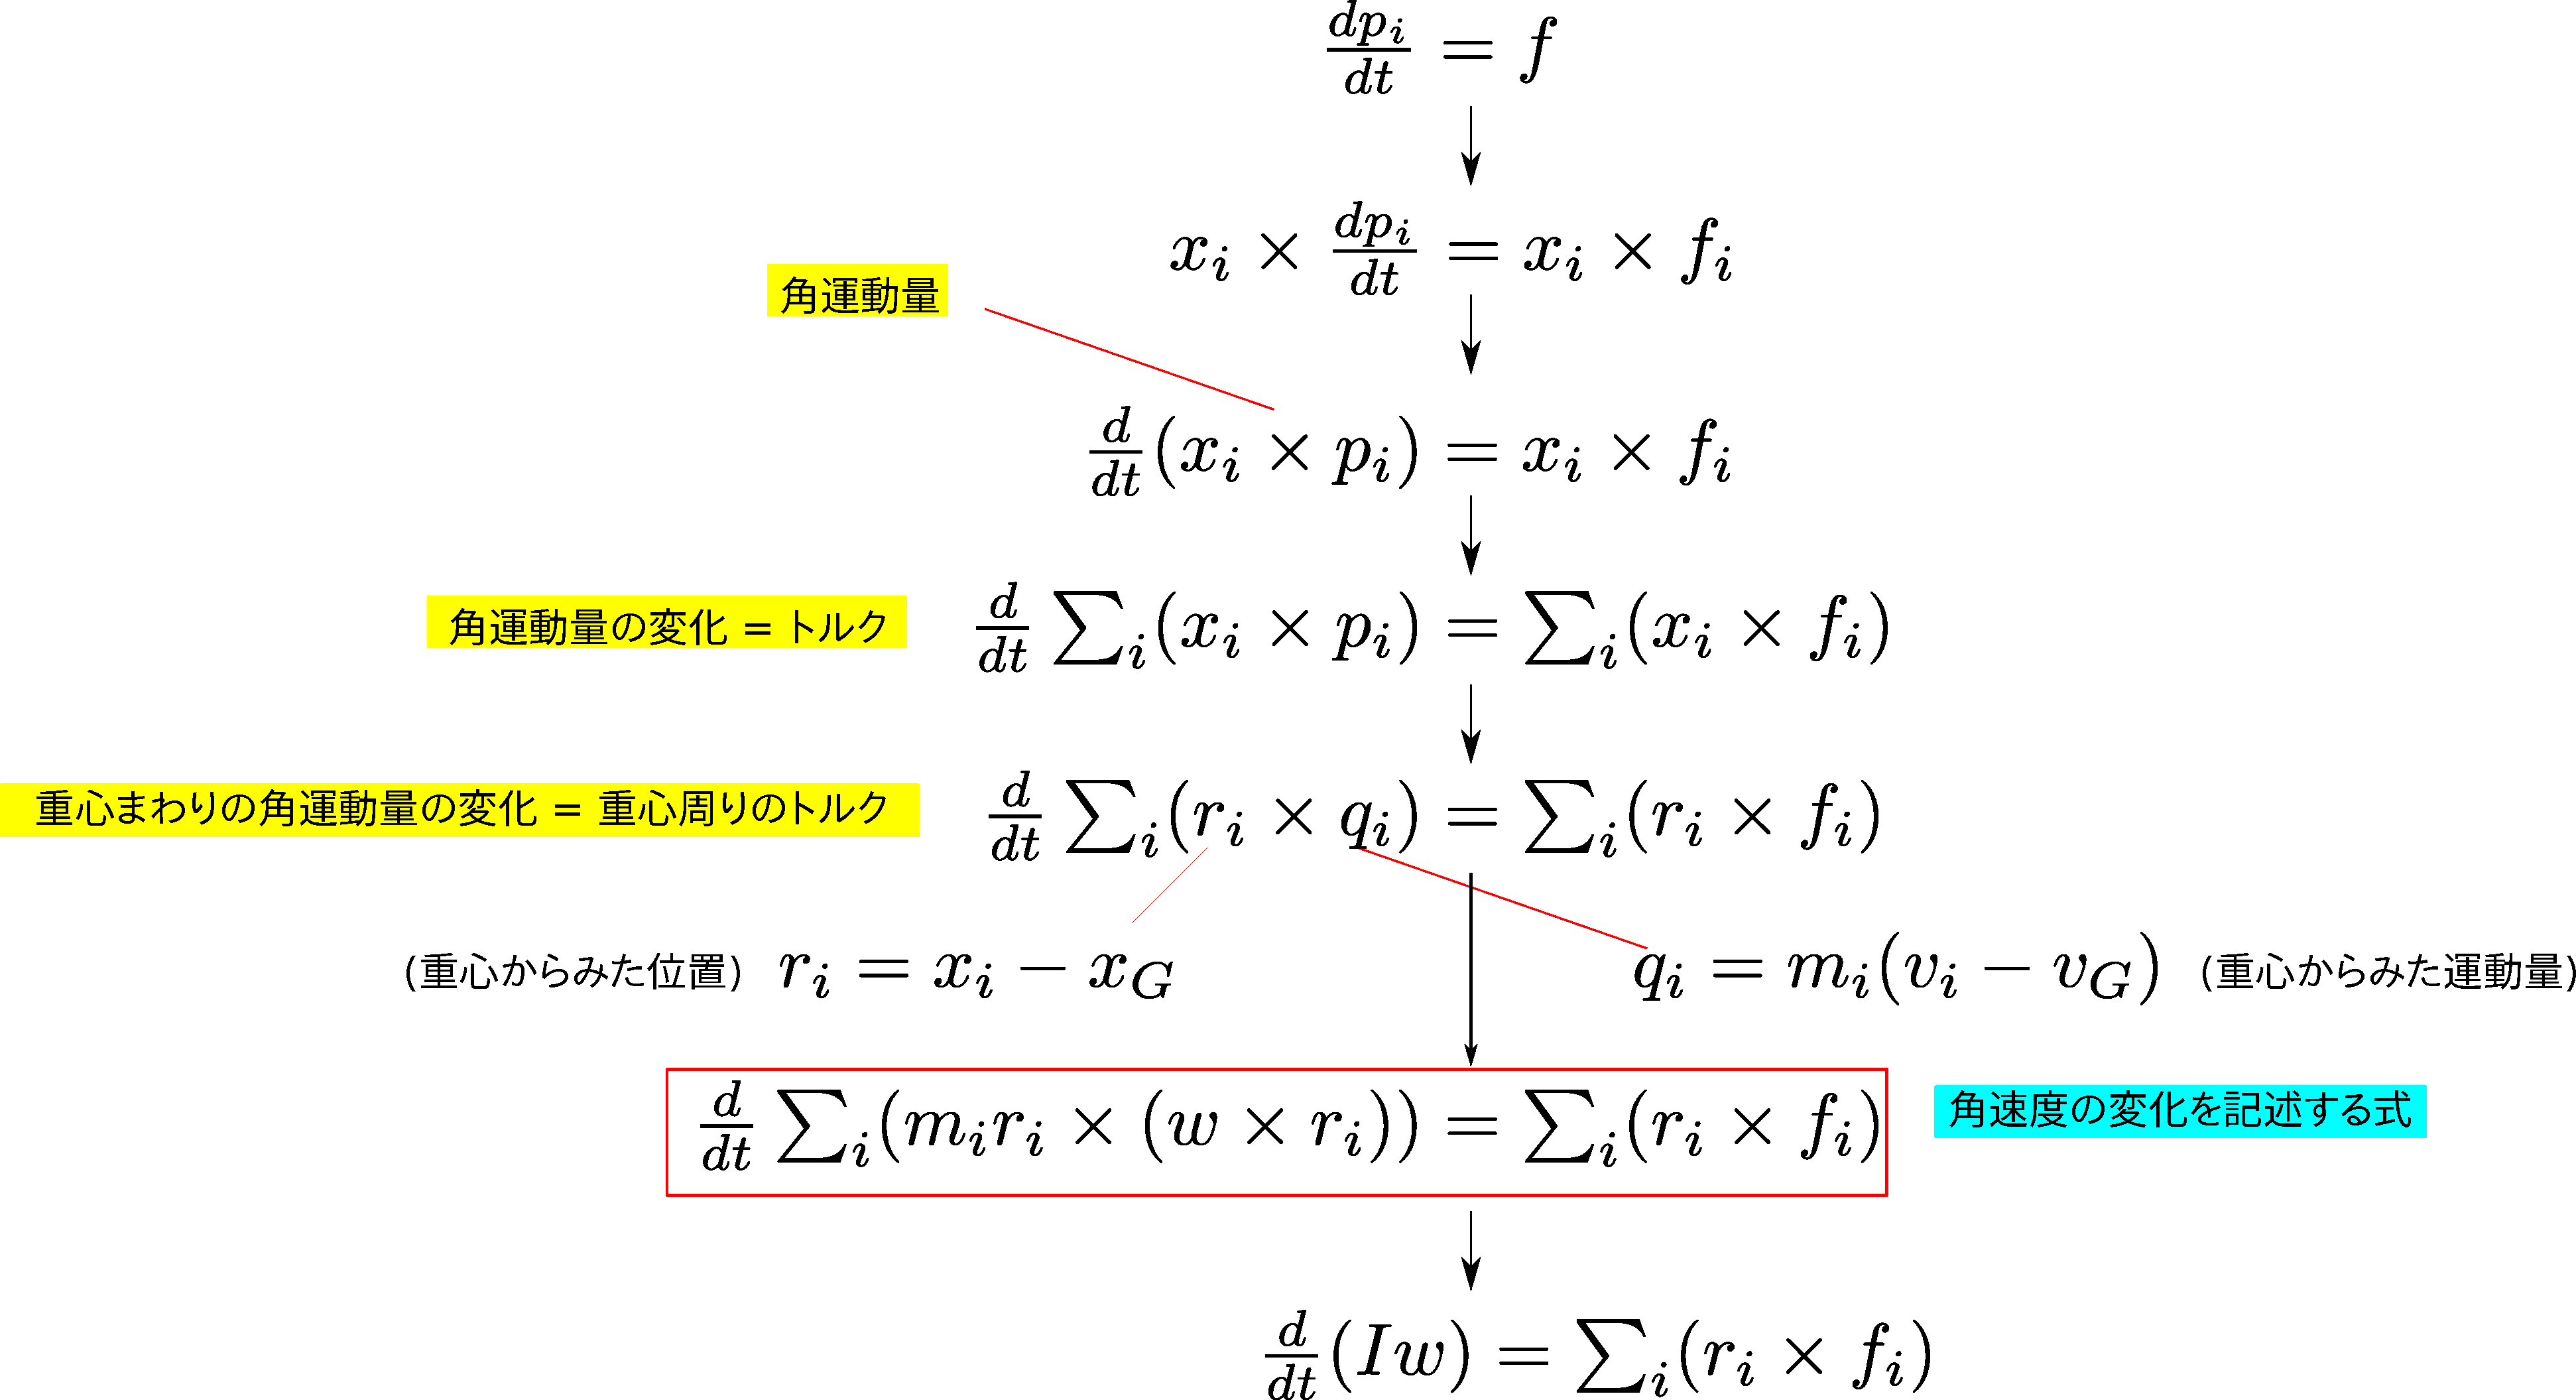
\includegraphics[width=\textwidth]{out/pdf/svg/rigid_roadmap.pdf}

次ページ以降, 各段階を詳し目に説明
\end{frame}


%%%%%%%%%%%%%%%%% %%%%%%%%%%%%%%%%% 
\begin{frame}
\frametitle{運動方程式 〜 角運動量}

\begin{itemize}
\item [] 質点$i$の運動方程式:
\begin{equation}
\frac{dp_i}{dt} = f_i
\end{equation}

\item [] 両辺に$x_i \times$ を施す:
\begin{equation}
x_i \times \frac{dp_i}{dt} = x_i \times f_i
\end{equation}

\item [] 
\begin{equation}
\therefore \frac{d}{dt}(x_i \times p_i) = x_i \times f_i \label{eq:angular}
\end{equation}
($\because \frac{d}{dt}(x_i \times p_i) = 
\frac{dx_i}{dt} \times p_i + x_i \times \frac{dp_i}{dt}
= p_i \times p_i + x_i \times \frac{dp_i}{dt}
= x_i \times \frac{dp_i}{dt}$)

\item []

\begin{itemize}
\item 「位置 $\times$ 運動量(上記の$(x_i \times p_i)$)」を\ao{「角運動量」}という
\item 「位置 $\times$ 力(上記の$x_i \times f_i$)」を\ao{「トルク」}という
\item 要するに, \ao{角運動量の時間変化 $=$ トルク} ということ
\end{itemize}
\end{itemize}
\end{frame}


%%%%%%%%%%%%%%%%% %%%%%%%%%%%%%%%%% 
\begin{frame}
\frametitle{全各運動量の時間変化 $=$ 外力による全トルク}
\begin{itemize}
\item [] 式(\ref{eq:angular})を全ての点にわたって足す
  \begin{equation}
\frac{d}{dt}\sum_i (x_i \times p_i) = \sum_i (x_i \times f^{\mbox{ext}}_i)
\label{eq:angular_momentum_torque}    
  \end{equation}
\begin{itemize}
\item 前と同様, $f^{\mbox{ext}}_i$は外力で, 以降${}^{\mbox{ext}}$は省略
\item $\therefore$ \ao{全角運動量の時間変化 $=$ 外力による全トルク}
\end{itemize}

\item これで, 外力が「全角運動量」をどう変化させるかがわかった
\item \aka{あとは, 全角運動量と角速度の関係がわかれば良い}ことになる
\item そのための手がかりが, 角速度と「各点の速度」を結ぶ式(\ref{eq:v_w_r}).
再掲:
\[ v_i = v_G + w \times (x_i - x_G) \]
\item そこで, $x_i$を, 重心との相対位置を使って書き換えていくことにする
\end{itemize}
\end{frame}

%%%%%%%%%%%%%%%%% %%%%%%%%%%%%%%%%% 
\begin{frame}
\frametitle{重心からの相対位置で書き換え}
\begin{itemize}
\item [] 質点$i$の, 質量中心からの相対的な位置を$r_i$と書くことにする. つまり,
\[ x_i = x_G + r_i \]
\item [] すると, 式(\ref{eq:angular_momentum_torque})は,
\[ \frac{d}{dt}\sum_i ((x_G + r_i) \times p_i) = \sum_i ((x_G + r_i) \times f_i) \]
\item [] 一方
\begin{eqnarray*}
\frac{d}{dt}\sum_i (x_G \times p_i) = \sum_i (x_G \times f_i )
\end{eqnarray*}
なので(証明は易しい練習問題), 辺同士引き算し, $p_i = m_i v_i$を用いると,
\item []
\[ \frac{d}{dt} \sum_i (r_i \times m_i v_i) = \sum_i (r_i \times f_i) \]
\end{itemize}
\end{frame}

%%%%%%%%%%%%%%%%% %%%%%%%%%%%%%%%%% 
\begin{frame}
\frametitle{}
\begin{itemize}
\item [] これを,
\[ v_i = v_G + w \times r_i \]
を用いて書き換える
\item []
\begin{equation}
\frac{d}{dt} \sum_i (r_i \times m_i (v_G + w \times r_i)) = \sum_i (r_i \times f_i )
\label{eq:angular}
\end{equation}
\item []
\begin{eqnarray*}
\mbox{左辺} & = & 
\frac{d}{dt} \left(\left(\sum_i m_i r_i\right) \times v_G \right)
+ \frac{d}{dt} \sum_i (r_i \times m_i (w \times r_i))
\end{eqnarray*}
\item [] ここで, 上記の第一項$=0$である.

($\because
\sum_i m_i r_i
= \sum_i m_i (x_i - x_G)
= \sum_i (m_i x_i) - \left(\sum_i m_i\right) x_G
= M x_G - M x_G 
$)

\end{itemize}
\end{frame}


%%%%%%%%%%%%%%%%% %%%%%%%%%%%%%%%%% 
\begin{frame}
\frametitle{}
\begin{itemize}
\item []
よって, 式(\ref{eq:angular})から以下が導かれる
\begin{equation}
\aka{\frac{d}{dt} \sum_i (m_i r_i \times (w \times r_i)) = \sum_i (r_i \times f_i)}
\label{eq:angular2}
\end{equation}
\item [] この式が, \aka{力に対して$w$がどう変化するかを決める方程式}である
\end{itemize}
\end{frame}


%%%%%%%%%%%%%%%%% %%%%%%%%%%%%%%%%% 
\begin{frame}
\frametitle{頭に入れるべき結果}
\begin{itemize}
\item 
\[ \frac{d}{dt} \sum_i r_i \times m_i (w \times r_i) = \sum_i r_i \times f_i \]
\item 見た目はごついが内容はわかりやすい(覚えやすい)
\item $m_i (w \times r_i)$は, 「重心から見た時の点$i$の運動量」. つまり上式は,
\begin{itemize}
\item [] \ao{「重心から見た角運動量の時間変化」= 「重心周りのトルク」}
\end{itemize}
ということ

{\scriptsize
\item 注: この式を当たり前と思ってはいけない. 特に,
\begin{quote}
「角運動量の時間変化」= 「トルク」
\end{quote}
という, \ao{位置ベクトルの「基準点」をどこにとっても}成りたつ式において, 
「基準点」を質量中心にとっただけ(よって当たり前)というわけではない

\item 「基準点」が(加速度)運動していなければそれでよいが,
「基準点」が(加速度)運動している場合はそうはいかない

\item その「基準点」が質量中心であれば, それでも同じ式が成り立つという,
(自明ではない)事実を言っている
}
\end{itemize}
\end{frame}

%%%%%%%%%%%%%%%%% %%%%%%%%%%%%%%%%% 
\begin{frame}
\frametitle{慣性モーメント}
\begin{itemize}
\item [] 再掲:
\[ \frac{d}{dt} \sum_i (r_i \times m_i (w \times r_i)) = \sum_i (r_i \times f_i) \]
\item ここで左辺の和は, 
\aka{$w$に対して線形な式なので, 全体を「ある行列」$I$を用いて,
$Iw$と書くことができるはず}である:
\[ \therefore Iw \stackrel{\mbox{\scriptsize def}}{\equiv} 
\sum_i (r_i \times m_i (w \times r_i)) \]

\item この行列$I$自身は$w$によらず, $m_i$と$r_i$, 
つまり, 剛体の各点が重心から見てがどのような位置にあるか---言い換えれば剛体全体の,
「姿勢」---だけから決まる

\item この行列を「慣性モーメント」と呼ぶ
\end{itemize}
\end{frame}


%%%%%%%%%%%%%%%%% %%%%%%%%%%%%%%%%% 
\begin{frame}
\frametitle{}
これまでの議論で, つまり以下のことがわかった

\begin{itemize}
\item 剛体の姿勢(だけ)から決まる, 「慣性モーメント」なる行列$I$があり,
\[ \frac{d}{dt}(Iw) = \sum_i (r_i \times f_i) \]
なる関係がある

\item これを用いると, 力がどのように角速度を変化させるかがわかる!

\[ \Delta w \approx I^{-1} \sum_i (r_i \times f_i) \Delta t\]
\end{itemize}
\end{frame}


%%%%%%%%%%%%%%%%% %%%%%%%%%%%%%%%%% 
\begin{frame}
\frametitle{慣性モーメントの計算}
\begin{itemize}
\item 先に, 
\[ \sum_i r_i \times m_i (w \times r_i) \]
の\aka{「\ldots 和は, $w$に対して線形な式なので, 
全体を「ある行列」$I$を用いて, $Iw$と書くことができるはずである」}
ということで $I$を定義したが,
これだけでは実際の形がイメージできないので実際に計算しておく.
\item もちろんシミュレーションにおいても計算する必要がある
\item 上記の一つの項を取り出し添字を省略したもの:
\[ r \times m (w \times r) \]
を実際に成分計算してみる. 
\end{itemize}
\end{frame}

%%%%%%%%%%%%%%%%% %%%%%%%%%%%%%%%%% 
\begin{frame}
\frametitle{慣性モーメントの計算}
\begin{itemize}
\item 
$r = (r_x, r_y, r_z)$, $w = (w_x, w_y, w_z)$と書くと,
\begin{eqnarray*}
& = & r \times m (w \times r)  \\
& = & m(r \cdot r) w - m(r \cdot w) r \\
& = & 
m\left(
\begin{array}{ccc}
r_x^2 + r_y^2 + r_z^2 &       & \\
     &  r_x^2 + r_y^2 + r_z^2  & \\
     &       & r_x^2 + r_y^2 + r_z^2 
\end{array}
\right) w \\
&  & 
- 
m\left(
\begin{array}{ccc}
r_x^2   & r_xr_y & r_xr_z \\
r_xr_y  & r_y^2  & r_yr_z \\
r_xr_z  & r_yr_z & r_z^2
\end{array}
\right)w \\
& = &
\ao{m\left(
\begin{array}{ccc}
r_y^2 + r_z^2 & -r_xr_y        & -r_zr_x \\
-r_xr_y      &  r_x^2 + r_z^2  & -r_yr_z \\
-r_xr_z      &  -r_yr_z        & r_x^2 + r_y^2
\end{array}
\right)} w
\end{eqnarray*}
\end{itemize}

これ\ao{(青字部分)}を全ての点について足したものが剛体の慣性モーメント
\end{frame}

%%%%%%%%%%%%%%%%% %%%%%%%%%%%%%%%%% 
\begin{frame}
\frametitle{慣性モーメント: 2次元の場合}
\begin{itemize}
\item 角速度ベクトルは$z$軸に平行 $\Rightarrow w = (0, 0, w)$と書ける
\item 位置ベクトルは$xy$平面内のベクトル $\Rightarrow r_z = 0$
\end{itemize}
よって,
\[
m\left(
\begin{array}{ccc}
r_y^2 + r_z^2 & -r_xr_y        & -r_zr_x \\
-r_xr_y      &  r_x^2 + r_z^2  & -r_yr_z \\
-r_xr_z      &  -r_yr_z        & r_x^2 + r_y^2
\end{array}
\right) w
= 
\left(\begin{array}{c}
0 \\ 0 \\ m(r_x^2 + r_y^2) w
\end{array}\right)
\]
つまり慣性モーメントは, 
\aka{$(\mbox{質量} \cdot \mbox{重心までの距離}^2)$}
を全ての点に渡って足したもの

\end{frame}

%%%%%%%%%%%%%%%%% %%%%%%%%%%%%%%%%% 
\begin{frame}
\frametitle{例: 2質点をつないだバトン}
\begin{columns}
\begin{column}{0.6\textwidth}
\begin{itemize}
\item 質量$m_1$と質量$m_2$の質点を長さ$l$の棒でつないだ
\item それを, ある平面内で回転させたときの慣性モーメント
\[ m_1 l_1^2 + m_2 l_2^2 \]
\item ここで$l_1$, $l_2$はそれぞれの点の重心からの距離で,
\[ l_1 = \frac{m_2}{m_1+m_2}l \]
\[ l_2 = \frac{m_1}{m_1+m_2}l \]
\end{itemize}
\end{column}

\begin{column}{0.4\textwidth}
\begin{center}
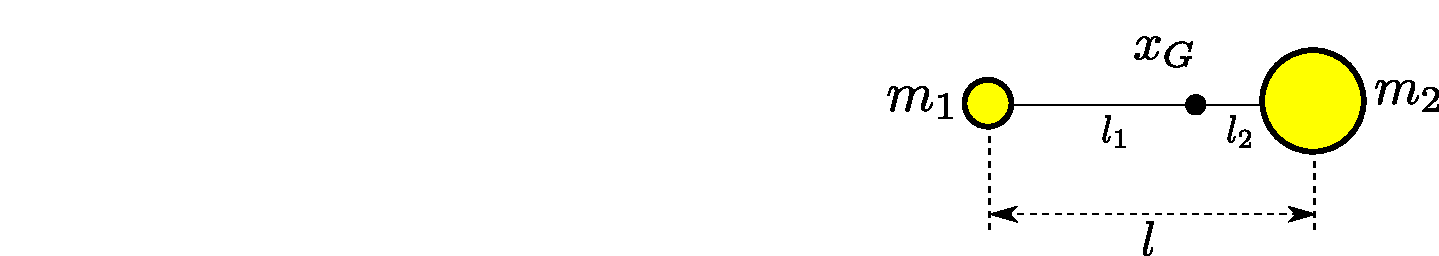
\includegraphics[width=0.8\textwidth]{out/pdf/svg/baton2.pdf}
\end{center}
\end{column}
  
\end{columns}

\end{frame}

%%%%%%%%%%%%%%%%% %%%%%%%%%%%%%%%%% 
\begin{frame}[fragile]
\frametitle{}
\begin{itemize}
\item 以上が, 「剛体の運動方程式」
\item それを元にした剛体運動追跡 
$=$ 質量中心と角速度追跡のテンプレート:
\begin{lstlisting}
n_steps = ステップ数
dt = (@\ao{終了時刻}@ - @\ao{開始時刻}@) / n_steps # 時間の刻み幅
xg = @\ao{質量中心の初期位置}@
vg = @\ao{質量中心の初速}@
w = @\ao{初期角速度}@
t = @\ao{開始時刻}@
for i in range(n_steps):
    f = @\aka{外力の和($\sum_i f_i$)}@
    tau = @\aka{外力によるトルクの和($\sum_i r_i \times f_i$)}@
    xg += vg * dt
    vg += f / M * dt
    w  += @${\tt I}^{-1}$@ tau * dt
    t += dt
\end{lstlisting}

\item 簡単のため, 積分はオイラー法. もちろんルンゲクッタ法も適用可能
\end{itemize}

\end{frame}


%%%%%%%%%%%%%%%%% %%%%%%%%%%%%%%%%% 
\begin{frame}[fragile]
\frametitle{アニメーション}
\begin{lstlisting}
n_steps = ステップ数
dt = (@\ao{終了時刻}@ - @\ao{開始時刻}@) / n_steps # 時間の刻み幅
xg = @\ao{質量中心の初期位置}@
vg = @\ao{質量中心の初速}@
w = @\ao{初期角速度}@
t = @\ao{開始時刻}@
for i in range(n_steps):
    f = @\aka{外力の和($\sum_i f_i$)}@
    tau = @\aka{外力によるトルクの和($\sum_i r_i \times f_i$)}@
    xg += vg * dt
    vg += f / M * dt
    w  += @${\tt I}^{-1}$@ tau * dt
    t += dt
\end{lstlisting}

\begin{itemize}
\item {\tt vg, w}がわかれば, 式(\ref{eq:v_w_r})を用いて,
各質点の速度がわかる
\item 速度がわかれば位置がわかる
\item これを利用してアニメーションなりなんなりをすればよい
\end{itemize}
\end{frame}

%%%%%%%%%%%%%%%%% %%%%%%%%%%%%%%%%% 
\begin{frame}[fragile]
\frametitle{衝突は?}
\begin{itemize}
\item ここまでは衝突がなく, 「スムースに」加速する場合の話

\item 衝突がある場合, 衝突の瞬間に起こるミクロな現象(分子間力による反発
  など)を全て再現できれば,「原理的には」これまでと同じ仕組みで再現でき
  るわけだが, そんなことはできない


\end{itemize}

\end{frame}

%%%%%%%%%%%%%%%%% %%%%%%%%%%%%%%%%% 
\begin{frame}[fragile]
\frametitle{衝突}

\begin{itemize}
\item 質量中心の運動と, 角速度の変化を追えば良いという考え方自体はここでも同じ

\item それらを積分する際に, 「各瞬間の力」が詳細にわからないのが問題

\item 質点が壁に跳ね返るような単純な場合でもこのへんの事情は同じ

\item ではこれまでどうしていたか? 
  \begin{itemize}
  \item $ma = f$を「衝突している間積分した式」を考えた
  \item $\Rightarrow$ 衝突時に受けた力積(力を時間で積分したもの)が, 運動量の変化になる
  \end{itemize}
\item この延長で考える
\end{itemize}
\end{frame}

%%%%%%%%%%%%%%%%% %%%%%%%%%%%%%%%%% 
\begin{frame}[fragile]
\frametitle{衝突}

\begin{itemize}
\item \ao{(運動量の変化 $=$ 力積)}:
\begin{eqnarray}
\frac{dp}{dt} = f 
& \Rightarrow & \int_{t_0}^{t_1} \frac{dp}{dt}dt = \int_{t_0}^{t_1} f dt \\
& \Rightarrow & \ao{p(t_1) - p(t_0) = \underline{\int_{t_0}^{t_1} f dt}}
\label{eq:a}
\end{eqnarray}

\item \ao{(角運動量の変化 $=$ 位置 $\times$ 力積)} {\scriptsize (「トルク積」という言葉があれば\ldots)}
\begin{eqnarray}
\frac{d}{dt}(Iw) = r \times f 
& \Rightarrow & \int_{t_0}^{t_1} \frac{d}{dt}(Iw)dt = \int_{t_0}^{t_1} r \times f dt \\
& \Rightarrow & 
\ao{I (w(t_1) - w(t_0)) = r \times \underline{\int_{t_0}^{t_1} f dt}}
\label{eq:b}
\end{eqnarray}

\end{itemize}
\end{frame}

%%%%%%%%%%%%%%%%% %%%%%%%%%%%%%%%%% 
\begin{frame}[fragile]
\frametitle{}
\begin{itemize}
\item ここまでのところは, 
質量中心の運動および角速度を追跡するために用いていた式を積分したもので,
衝突であろうとなかろうと成り立つ

\item 「力積」がいくらになるかが残された未知数で, 
本当は衝突のミクロなメカニズムによって決まるのだが, 
それを再現することはできないので, 経験的な式を用いる.

\item $\Rightarrow$ 反発係数
\end{itemize}
\end{frame}

%%%%%%%%%%%%%%%%% %%%%%%%%%%%%%%%%% 
\begin{frame}[fragile]
\frametitle{衝突に関する経験的な法則}
\begin{columns}
\begin{column}{0.5\textwidth}
\begin{itemize}
\item さしあたり, 動かない平面壁との衝突を考える
\item 壁の法線ベクトル(長さ1, 向きは物体がある向き)を$n$とする
\end{itemize}
\end{column}
\begin{column}{0.5\textwidth}
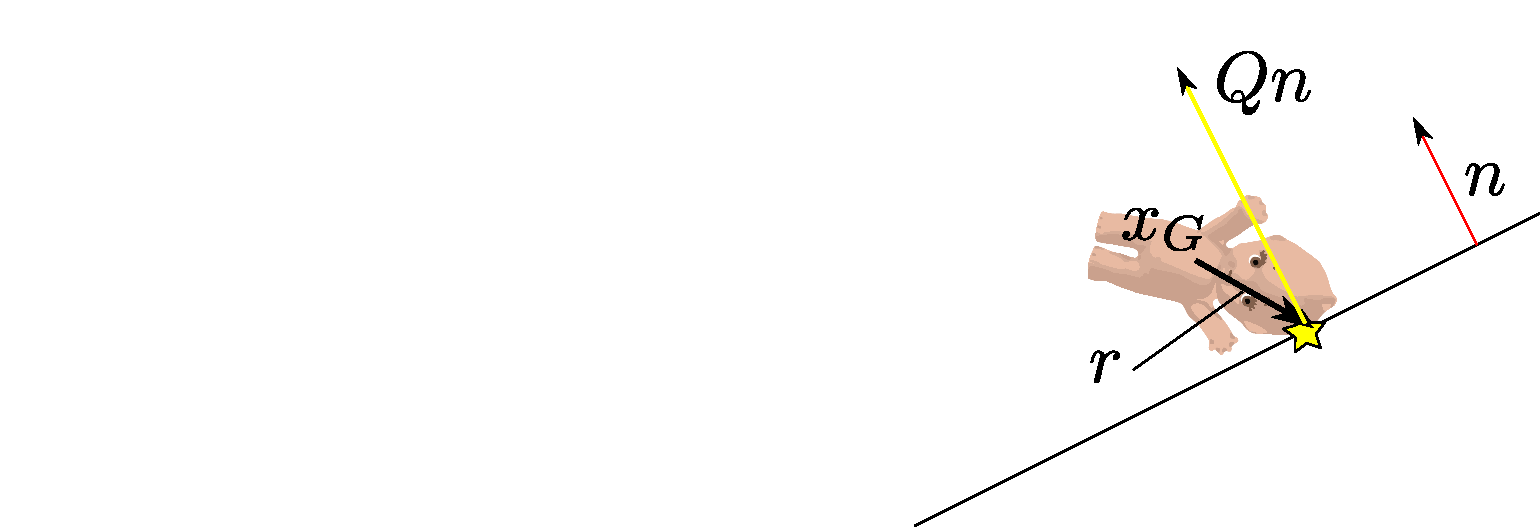
\includegraphics[width=\textwidth]{out/pdf/svg/collision_with_wall.pdf}
\end{column}  
\end{columns}

\begin{itemize}
\item この設定のもとで, 
\begin{equation}
\ao{
\frac{\mbox{{\bf 衝突した点における}剛体の速度(衝突後)の$n$方向の成分} }
{\mbox{{\bf 衝突した点における}剛体の速度(衝突前)の$n$方向の成分} }
= - \mbox{反発係数}}
\label{eq:c}
\end{equation}

\item 力積の方向は$n$ (未知数は大きさだけ)
\item 式(\ref{eq:a}), (\ref{eq:b}), (\ref{eq:c})を連立させることで, 衝突後の$v_G$, $w$が求まる
\end{itemize}
\end{frame}


%%%%%%%%%%%%%%%%% %%%%%%%%%%%%%%%%% 
\begin{frame}[fragile]
\frametitle{具体的な計算}
\begin{itemize}
\item 衝突前の質量中心の速度, 角速度を$v_G$, $w$,
\item 衝突後の質量中心の速度, 角速度を$v'_G$, $w'$とする
\item 衝突時に受けた力積の大きさを$Q$とする(方向および向きは$n$)
\end{itemize}

\begin{itemize}
\item 条件(\ref{eq:a}):
\begin{equation}
M (v'_G - v_G) = Q n \label{eq:aa}
\end{equation}
\item 条件(\ref{eq:b}):
\begin{equation}
I (w' - w_G) = r \times Q n \label{eq:bb}
\end{equation}
($r$は質量中心から衝突点までのベクトル)
\item 条件(\ref{eq:c}):
\begin{equation}
\frac{(v'_G + w' \times r) \cdot n}{(v_G + w \times r) \cdot n} = -e
\label{eq:cc}
\end{equation}
\end{itemize}
以上の, $v'_G, w', Q$に関する連立方程式を(3つの方程式で)解く
\end{frame}


%%%%%%%%%%%%%%%%% %%%%%%%%%%%%%%%%% 
\begin{frame}[fragile]
\frametitle{}
\begin{itemize}
\item 式(\ref{eq:aa})より,
\[ v'_G = v_G +  Q/M n \]
\item 式(\ref{eq:bb})より,
\[ w' = w + QI^{-1} (r \times n) \]
\item これを式(\ref{eq:cc})に代入
\[ 
(v_G +  Q/M n + (w + QI^{-1} (r \times n)) \times r) \cdot n
= -e ((v_G + w \times r) \cdot n)
\]
\item 目が眩みそうになるが落ち着いて. もはや未知数は$Q$というスカラー一つのみ.
$Q$を括りだせば自ずと道は開かれる
\item []
\[ 
(v_G +(w \times r)) \cdot n +  Q/M + Q (((I^{-1} (r \times n)) \times r) \cdot n)
= -e ((v_G + w \times r) \cdot n)
\]

\[ 
\therefore (1 + e) (v_G +(w \times r)) \cdot n 
= -Q (1/M + (((I^{-1} (r \times n)) \times r) \cdot n))
\]

\[ 
\therefore Q = 
-(1 + e) \frac{(v_G +(w \times r)) \cdot n}{(1/M + ((I^{-1} (r \times n)) \times r) \cdot n)}
\]

\end{itemize}
\end{frame}

%%%%%%%%%%%%%%%%% %%%%%%%%%%%%%%%%% 
\begin{frame}[fragile]
\frametitle{最後の注}

\begin{itemize}
\item 以上が, かなり一般的な剛体の運動のシミュレーションの仕方

\item ここで述べた方法は, 複雑な物体の3次元内の運動に対してそのまま適用できる
  \begin{itemize}
  \item 慣性モーメントさえ計算できれば物体の形状や点の数は問わない
  \item 人形やコマなど質量が連続的に分布していても,
    適宜積分を使えば慣性モーメントは計算できる
  \end{itemize}

\item 問題19では色々な意味で, 衝突以外の運動に大した面白みはない
  \begin{itemize}
  \item 重心周りのトルク$=0 \Rightarrow$ 角速度は変化しない
  \item 運動が2次元内に収まっている
  \end{itemize}

\item それでもプログラム上は, 
  このような一般的な定式化に沿ったもののほうが簡単だったりする

\item $I^{-1}$を計算するところはプログラミングは難しい(連立一次方程式を解く). 
  後に出てくる numpy を使えば一発

\item また, 衝突は壁との衝突のみだったが, 
  ここでの扱いを少し修正すれば物体同士の衝突も扱える
\end{itemize}
\end{frame}

%%%%%%%%%%%%%%%%% %%%%%%%%%%%%%%%%% 
\begin{frame}[fragile]
\frametitle{個人的雑感}
シミュレーションもこのくらいになると, 
\aka{少し難しい物理を生き生きと理解する}助けになる例と期待しています

\begin{itemize}
\item 自分の物理の理解が間違っていると, 
  コンピュータ(アニメーション)がそれを間違っていると教えてくれる

\item 一方, アニメーションがおかしいとき, それがコーディングのミスなのか,
  物理のミスなのかを知るのは難しい

\item そこで「物理は間違っていない」と
  自信を持って言えるようでないと安心してコーディングにのぞめない

\item $\Rightarrow$ シミュレーションをすると,
「物理をごまかしなく, しっかりと理解する」はめになる

\item 個人的には, こういう機会でもなければ,
  剛体の物理など, ここまで厳密に理解する気が起きない
  \footnote{もちろん物理学科や物理工学科の人はそうではないのでしょうけれど\ldots}

\end{itemize}


\end{frame}

\end{document}
